\chapter{ファイル拡張子とプログラミング言語}

\section{この章で学ぶこと}

GitHubでリポジトリを眺めていると、\cmd{.py}、\cmd{.js}、\cmd{.yaml}、\cmd{.md} など、実にさまざまな拡張子を持つファイルが並んでいることに気づきます。プログラミング経験がない人にとって、これらのファイルが何を意味するのかを理解することは、リポジトリの全体像を把握するための第一歩です。

この章では、以下の内容を学びます。

\begin{itemize}
  \item ファイル拡張子の基本的な役割と、GitHubでの表示への影響
  \item 主要なプログラミング言語とそれに対応する拡張子
  \item データファイルや設定ファイルに使われる拡張子の種類と使い分け
  \item ドキュメントファイルの拡張子
  \item ビルドやパッケージ管理に使われるファイル
  \item GitHub特有のファイルやディレクトリの役割
  \item GitHubがリポジトリの言語を判定する仕組み
  \item 文字コードの基礎知識
  \item 拡張子を持たないファイルの意味
\end{itemize}

この章は「プログラミング言語の入門」ではなく、「GitHubのリポジトリを読み解くための地図」として活用してください。それぞれの拡張子がどのような文脈で使われるのかを知ることで、初めて見るリポジトリでも「このプロジェクトは何の技術で作られているのか」が一目で判断できるようになります。

\section{拡張子とは何か}

\subsection{ファイル名の末尾の .xxx の役割}

ファイルの\textbf{拡張子}とは、ファイル名の末尾にあるピリオド以降の部分のことです。たとえば \cmd{report.pdf} というファイル名であれば、\cmd{.pdf} が拡張子です。

\begin{lstlisting}[language={}]
main.py       ← .py = Pythonで書かれたプログラム
index.html    ← .html = Webページの構造を記述したファイル
style.css     ← .css = Webページの見た目を定義したファイル
README.md     ← .md = Markdownで書かれた文書
data.csv      ← .csv = カンマ区切りの表データ
\end{lstlisting}

拡張子の役割は、\textbf{このファイルがどのような種類のデータを含んでいるか}をコンピュータと人間の両方に伝えることです。OSはファイルの拡張子を見て、どのアプリケーションでファイルを開くかを判断します。テキストエディタはファイルの拡張子を見て、どのプログラミング言語のルールで色分けするかを決定します。

\subsection{GitHubでのシンタックスハイライト}

GitHubでは、ファイルの拡張子に基づいて\textbf{シンタックスハイライト}（構文の色分け表示）が自動的に適用されます。たとえば、\cmd{.py} ファイルを開くと、Pythonの予約語（\cmd{def}、\cmd{class}、\cmd{import} など）が青色で、文字列が緑色で、コメントがグレーで表示されます。

\begin{figure}[htbp]
\centering
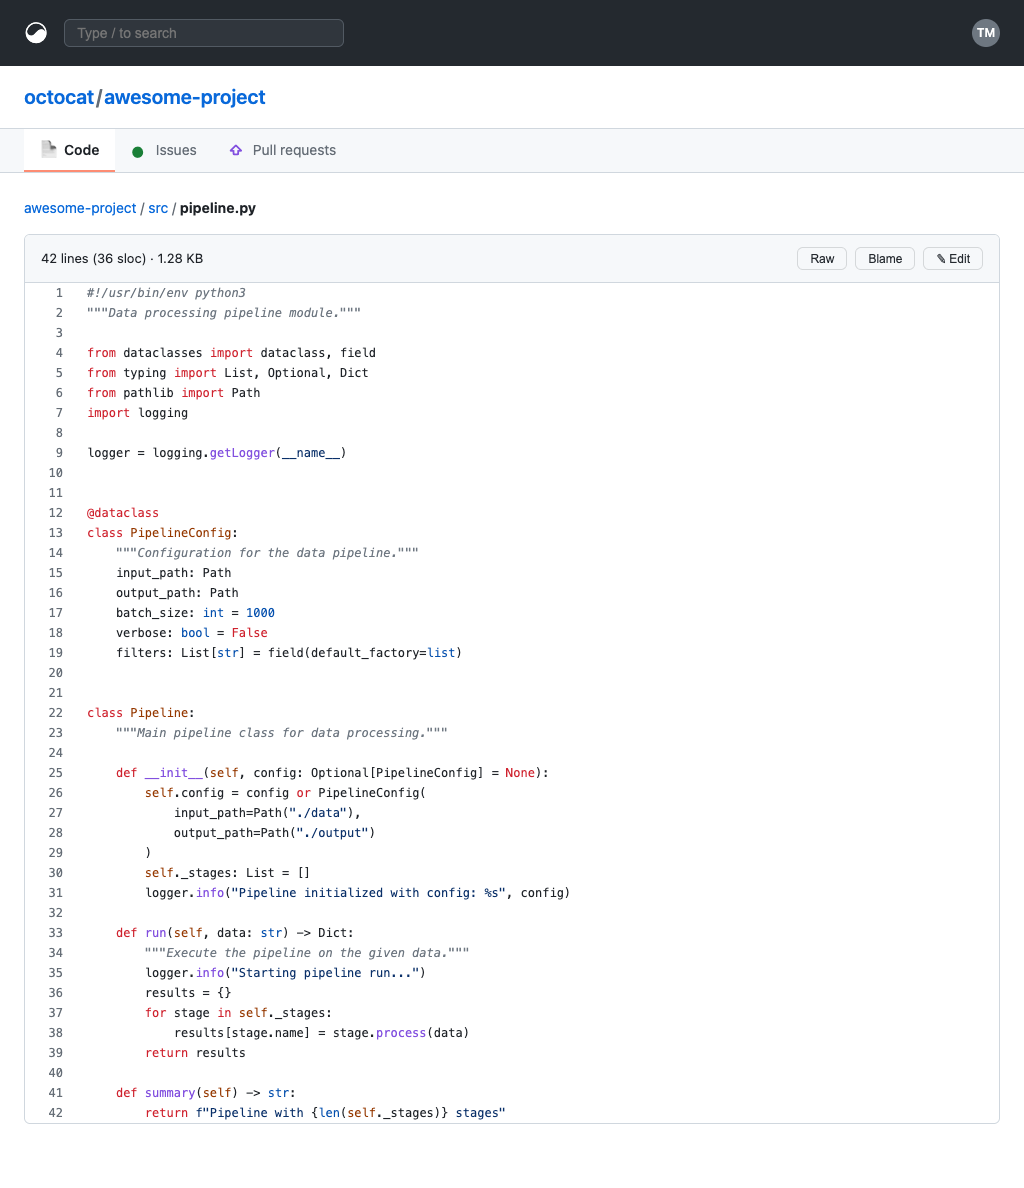
\includegraphics[width=0.95\textwidth]{images/syntax-highlight.png}
\caption{GitHubでのPythonファイルのシンタックスハイライト表示}
\end{figure}

この色分けのおかげで、コードの構造が一目で把握しやすくなります。もし拡張子がないファイルや、GitHubが認識できない拡張子のファイルの場合は、色分けされずにプレーンテキストとして表示されます。

\section{プログラミング言語と拡張子}

\subsection{Web開発の拡張子}

Web開発は、複数の言語を組み合わせて行います。それぞれの言語が異なる役割を担っています。

\begin{table}[h]
\centering
\begin{tabular}{llll}
\hline
拡張子 & 言語/技術 & 役割 & 具体例 \\
\hline
\cmd{.html} & HTML & Webページの構造（骨格） & \cmd{index.html} \\
\cmd{.css} & CSS & Webページの見た目（装飾） & \cmd{style.css} \\
\cmd{.js} & JavaScript & Webページの動的な振る舞い & \cmd{app.js} \\
\cmd{.ts} & TypeScript & JavaScriptに型の安全性を追加した言語 & \cmd{app.ts} \\
\cmd{.jsx} & JSX & React（UIライブラリ）用のJavaScript & \cmd{App.jsx} \\
\cmd{.tsx} & TSX & React用のTypeScript & \cmd{App.tsx} \\
\cmd{.vue} & Vue.js & Vue.jsフレームワークのコンポーネント & \cmd{Header.vue} \\
\cmd{.svelte} & Svelte & Svelteフレームワークのコンポーネント & \cmd{App.svelte} \\
\cmd{.php} & PHP & サーバーサイドのWeb開発言語 & \cmd{index.php} \\
\cmd{.scss} / \cmd{.sass} & Sass & CSSをより効率的に書くための拡張言語 & \cmd{main.scss} \\
\hline
\end{tabular}
\end{table}

HTMLは家の骨組み、CSSは壁紙や家具の配置、JavaScriptは電気系統（スイッチを押すと照明が点く）にたとえることができます。Web開発のリポジトリでこれらの拡張子を見かけたら、「ああ、Webサイトやアプリを作っているプロジェクトだな」と判断できます。

TypeScript（\cmd{.ts}）はJavaScriptの拡張版で、変数の型を明示的に宣言できるようにした言語です。大規模なプロジェクトではバグの防止に役立つため、近年は \cmd{.js} よりも \cmd{.ts} を使うプロジェクトが増えています。

\subsection{汎用プログラミング言語の拡張子}

Web開発に限らず、さまざまな用途で使われる汎用的なプログラミング言語の一覧です。

\begin{table}[h]
\centering
\begin{tabular}{llll}
\hline
拡張子 & 言語 & 特徴 & 主な用途 \\
\hline
\cmd{.py} & Python & 読みやすく書きやすい & AI/ML、データ分析、Web開発、自動化スクリプト \\
\cmd{.java} & Java & エンタープライズ向けの堅牢な言語 & 業務システム、Androidアプリ \\
\cmd{.go} & Go & Googleが開発した高速な言語 & サーバー、CLI、インフラツール \\
\cmd{.rs} & Rust & メモリ安全性と高速性を両立 & システム開発、WebAssembly \\
\cmd{.rb} & Ruby & 書きやすさを重視した言語 & Web開発（Ruby on Rails） \\
\cmd{.swift} & Swift & Appleが開発した言語 & iOS / macOS アプリ \\
\cmd{.kt} & Kotlin & Javaの後継となるモダンな言語 & Androidアプリ、サーバー \\
\cmd{.c} & C言語 & 低レベルで高速な言語 & OS、組み込みシステム \\
\cmd{.cpp} / \cmd{.cc} & C++ & C言語を拡張した言語 & ゲームエンジン、システム開発 \\
\cmd{.h} & C/C++ ヘッダー & 関数や型の宣言を記述 & ライブラリのインターフェース定義 \\
\cmd{.cs} & C\# & Microsoft製の言語 & ゲーム（Unity）、Windows アプリ \\
\cmd{.dart} & Dart & Google製の言語 & Flutter（クロスプラットフォームアプリ） \\
\cmd{.scala} & Scala & JVM上で動く関数型言語 & ビッグデータ処理（Apache Spark） \\
\cmd{.ex} / \cmd{.exs} & Elixir & 並行処理に強い言語 & 高負荷Webサーバー \\
\cmd{.lua} & Lua & 軽量なスクリプト言語 & ゲームへの組み込み \\
\cmd{.pl} / \cmd{.pm} & Perl & テキスト処理に強い言語 & レガシーシステム \\
\hline
\end{tabular}
\end{table}

GitHubでリポジトリを見たとき、主に使われている拡張子からプロジェクトの性質を推測できます。\cmd{.py} ファイルが多ければPythonプロジェクト、\cmd{.go} ファイルが多ければGoのプロジェクト、\cmd{.rs} ファイルが多ければRustのプロジェクトです。

\subsection{データサイエンス・科学計算の拡張子}

データサイエンスやバイオインフォマティクスの分野では、独自の拡張子を持つファイルが多く使われます。

\begin{table}[h]
\centering
\begin{tabular}{lll}
\hline
拡張子 & 言語/形式 & 用途 \\
\hline
\cmd{.py} & Python & データ分析、機械学習 \\
\cmd{.R} / \cmd{.r} & R言語 & 統計分析、データの可視化 \\
\cmd{.Rmd} & R Markdown & Rのコードとレポートを統合した文書 \\
\cmd{.ipynb} & Jupyter Notebook & 対話型のデータ分析（Python/Rなど） \\
\cmd{.jl} & Julia & 高速な科学計算 \\
\cmd{.m} & MATLAB & 数値計算（大学や研究機関で多用） \\
\cmd{.nf} & Nextflow & バイオインフォマティクスのパイプライン記述 \\
\cmd{.wdl} & WDL & ワークフロー記述言語 \\
\cmd{.qza} / \cmd{.qzv} & QIIME 2 & メタゲノム解析のデータ（アーティファクト） \\
\hline
\end{tabular}
\end{table}

\cmd{.ipynb}（Jupyter Notebook）はGitHubで特別に対応されており、ノートブックの内容（コード、出力結果、グラフ）がそのままレンダリングされて表示されます。これは、コードと実行結果を一緒に確認できるため、データサイエンスのプロジェクトでは特に重宝されます。

\subsection{シェルスクリプトの拡張子}

シェルスクリプトは、コマンドラインで実行する一連のコマンドをファイルにまとめたものです。OSの種類やシェルの種類によって拡張子が異なります。

\begin{table}[h]
\centering
\begin{tabular}{lll}
\hline
拡張子 & 言語 & 用途 \\
\hline
\cmd{.sh} & Bash / Shell & Linux / macOS での自動化スクリプト \\
\cmd{.bash} & Bash & Bash専用のスクリプト \\
\cmd{.zsh} & Zsh & Zsh専用のスクリプト（macOSのデフォルトシェル） \\
\cmd{.fish} & Fish & Fishシェル用のスクリプト \\
\cmd{.ps1} & PowerShell & Windowsの高機能シェルスクリプト \\
\cmd{.bat} / \cmd{.cmd} & バッチファイル & Windowsのコマンドプロンプト用スクリプト \\
\hline
\end{tabular}
\end{table}

GitHubのリポジトリで \cmd{.sh} ファイルを見かけたら、ビルドスクリプト、デプロイスクリプト、セットアップスクリプトなど、何らかの自動化処理が含まれていると考えてよいでしょう。

\section{データ・設定ファイルの拡張子}

プログラミング言語のファイル以外にも、データや設定を記述するためのファイル形式が多数あります。それぞれの形式には特徴と得意分野があり、適材適所で使い分けられています。

\begin{table}[h]
\centering
\begin{tabular}{llll}
\hline
拡張子 & 形式名 & 特徴 & 主な用途 \\
\hline
\cmd{.json} & JSON & 構造化データの標準形式。プログラムから読み書きしやすい & APIのデータ交換、設定ファイル \\
\cmd{.yaml} / \cmd{.yml} & YAML & 人間にとって読み書きしやすい形式 & GitHub Actions、Docker Compose \\
\cmd{.toml} & TOML & セクション構造が明確で読みやすい & Rust（Cargo.toml）やPython（pyproject.toml） \\
\cmd{.xml} & XML & タグベースの構造化データ。冗長だが表現力が高い & Javaプロジェクトの設定（pom.xml） \\
\cmd{.csv} & CSV & カンマ区切りの表データ。最もシンプルな表形式 & データの受け渡し \\
\cmd{.tsv} & TSV & タブ区切りの表データ & バイオインフォマティクスのデータ \\
\cmd{.ini} / \cmd{.cfg} & INI & セクションとキー=値のシンプルな形式 & 古い設定ファイル \\
\cmd{.env} & 環境変数 & KEY=VALUE 形式の環境変数定義 & APIキーなどの秘密情報 \\
\hline
\end{tabular}
\end{table}

\textbf{\cmd{.env} ファイルには特に注意が必要です。} \cmd{.env} ファイルにはパスワードやAPIキーなどの秘密情報が含まれることが多いため、\textbf{必ず \cmd{.gitignore} に追加して、Gitの追跡対象から除外}してください。一度GitHubにプッシュしてしまった秘密情報は、コミット履歴に残り続けるため、すべてのキーやパスワードを無効化して再発行する必要があります。

JSONとYAMLは同じデータを異なる形式で表現できます。たとえば、同じデータをJSON形式で書くと波括弧とダブルクォーテーションが多くなりますが、YAML形式で書くとインデントだけで構造を表現するためスッキリします。人間が直接編集するファイル（設定ファイルなど）にはYAMLが好まれ、プログラム間のデータ交換にはJSONが好まれる傾向があります。

\section{ドキュメントファイルの拡張子}

ソフトウェアプロジェクトにはドキュメント（文書）が欠かせません。ドキュメントの形式もいくつかの種類があります。

\begin{table}[h]
\centering
\begin{tabular}{llll}
\hline
拡張子 & 形式名 & 特徴 & 主な用途 \\
\hline
\cmd{.md} & Markdown & シンプルな記法で見出し・リスト・リンクを表現できる & README、プロジェクトドキュメント \\
\cmd{.rst} & reStructuredText & Markdownより表現力が高い & Pythonプロジェクトの公式ドキュメント \\
\cmd{.txt} & プレーンテキスト & 書式なしの純粋なテキスト & LICENSE、簡単なメモ \\
\cmd{.adoc} & AsciiDoc & 高機能な文書作成形式 & 技術書、長い文書 \\
\cmd{.tex} & LaTeX & 数式や論文レイアウトに特化した組版言語 & 学術論文、技術報告書 \\
\cmd{.org} & Org Mode & Emacs向けの文書形式 & ノート、タスク管理 \\
\hline
\end{tabular}
\end{table}

GitHubでは \cmd{.md}（Markdown）ファイルが最もよく使われます。GitHubは Markdownファイルを自動的にレンダリング（見出し・太字・リンクなどを反映して整形表示）するため、リポジトリのトップページに \cmd{README.md} を配置するのが標準的な慣習です。

\section{ビルド・パッケージ管理ファイル}

ソフトウェアプロジェクトには、プログラムのビルド方法や依存ライブラリを定義するファイルが含まれています。これらのファイルを見ると、そのプロジェクトがどの言語やツールを使っているかがわかります。

\begin{table}[h]
\centering
\begin{tabular}{lll}
\hline
ファイル名 & 言語/ツール & 用途 \\
\hline
\cmd{Makefile} & Make & ビルド手順の定義（C/C++プロジェクトに多い） \\
\cmd{CMakeLists.txt} & CMake & クロスプラットフォーム対応のビルド設定 \\
\cmd{Dockerfile} & Docker & コンテナイメージの構築手順 \\
\cmd{docker-compose.yml} & Docker Compose & 複数のコンテナの構成を定義 \\
\cmd{package.json} & npm (Node.js) & JavaScriptプロジェクトの依存ライブラリと設定 \\
\cmd{requirements.txt} & pip (Python) & Pythonプロジェクトの依存ライブラリの一覧 \\
\cmd{pyproject.toml} & Python & 現代的なPythonプロジェクトの設定と依存関係 \\
\cmd{Cargo.toml} & Cargo (Rust) & Rustプロジェクトの設定と依存関係 \\
\cmd{go.mod} & Go Modules & Goプロジェクトの依存関係 \\
\cmd{Gemfile} & Bundler (Ruby) & Rubyプロジェクトの依存ライブラリ \\
\cmd{build.gradle} & Gradle (Java/Kotlin) & Java/Kotlinプロジェクトのビルド設定 \\
\cmd{pom.xml} & Maven (Java) & Javaプロジェクトのビルドと依存関係 \\
\cmd{Cargo.lock} / \cmd{package-lock.json} & 各種 & 依存ライブラリの正確なバージョンを固定するファイル \\
\hline
\end{tabular}
\end{table}

たとえば、リポジトリのルートに \cmd{package.json} があれば「Node.js（JavaScript/TypeScript）のプロジェクト」、\cmd{requirements.txt} か \cmd{pyproject.toml} があれば「Pythonのプロジェクト」、\cmd{Cargo.toml} があれば「Rustのプロジェクト」と判断できます。これらのファイルは、いわばプロジェクトの「名刺」のようなものです。

\section{GitHub特有のファイルとフォルダ}

GitHubでは、特定のファイル名やディレクトリ名を使うことで、GitHubの機能と連動する特別な動作を実現できます。

\subsection{リポジトリルートの特別なファイル}

\begin{table}[h]
\centering
\begin{tabular}{ll}
\hline
ファイル名 & 役割 \\
\hline
\cmd{README.md} & リポジトリのトップページに自動表示されるプロジェクト説明文 \\
\cmd{LICENSE} & プロジェクトのライセンス。GitHubがライセンスを自動認識する \\
\cmd{.gitignore} & Gitの追跡対象から除外するファイルのパターンを定義する \\
\cmd{.gitattributes} & ファイルの属性（改行コード、差分表示方法、LFS対象など）を定義する \\
\cmd{CLAUDE.md} & Claude Codeへのプロジェクト固有の指示を記述するファイル \\
\hline
\end{tabular}
\end{table}

\cmd{README.md} はリポジトリの「顔」であり、プロジェクトが何をするものなのか、どうやって使うのかを最初に伝える場所です。GitHubはリポジトリのトップページに \cmd{README.md} の内容を自動的にレンダリングして表示するため、丁寧に書かれた \cmd{README.md} は訪問者にとって非常に助けになります。

\subsection{.github/ ディレクトリ内の各種ファイル}

\cmd{.github/} ディレクトリは、GitHubの各種機能に関連する設定ファイルを格納する特別なディレクトリです。

\begin{table}[h]
\centering
\begin{tabular}{ll}
\hline
ファイル/ディレクトリ & 役割 \\
\hline
\cmd{.github/workflows/} & GitHub Actionsのワークフローファイル（YAMLファイル）を格納する \\
\cmd{.github/ISSUE\_TEMPLATE/} & Issue作成時のテンプレートを格納する \\
\cmd{.github/pull\_request\_template.md} & PR作成時に自動挿入されるテンプレート \\
\cmd{.github/CODEOWNERS} & ファイルやディレクトリごとのレビュー担当者を定義する \\
\cmd{.github/dependabot.yml} & Dependabot（依存ライブラリの自動更新）の設定 \\
\cmd{.github/FUNDING.yml} & リポジトリのスポンサーボタンの設定 \\
\hline
\end{tabular}
\end{table}

\cmd{.github/workflows/} ディレクトリにYAMLファイルが入っていれば、そのリポジトリではGitHub Actions（自動テストやデプロイ）が設定されていることがわかります。\cmd{.github/CODEOWNERS} があれば、PRを作成したときに自動的に適切なレビュアーがアサインされる仕組みが導入されています。

\section{GitHubの言語判定の仕組み}

\subsection{linguistによる自動判定}

GitHubのリポジトリページには、使用されているプログラミング言語の割合を示すカラーバーが表示されます。「Python 65\%、JavaScript 25\%、Shell 10\%」のように、各言語が色分けされたバーで視覚的に表現されます。

\begin{figure}[htbp]
\centering
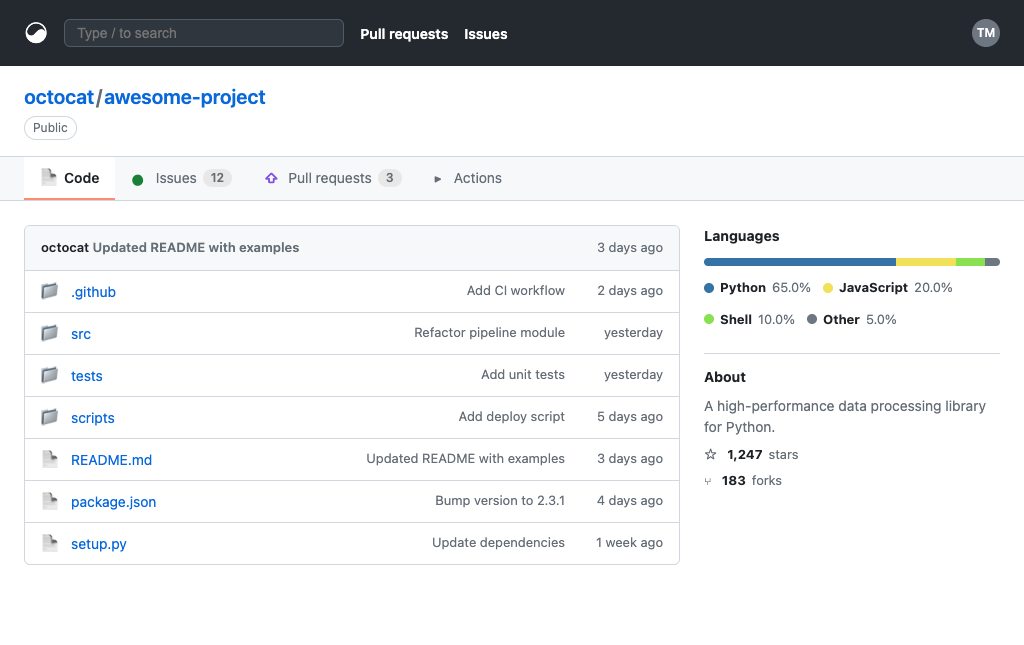
\includegraphics[width=0.95\textwidth]{images/language-bar.png}
\caption{GitHubリポジトリの言語バー}
\end{figure}

この言語判定は、\textbf{Linguist}（https://github.com/github-linguist/linguist）というオープンソースのツールによって行われています。Linguistはリポジトリ内の全てのファイルを解析し、拡張子やファイルの内容に基づいて使用言語を判定します。

ただし、Linguistの判定には以下のルールがあります。

\begin{itemize}
  \item \cmd{vendor/} ディレクトリ内のファイルは「外部ライブラリ」とみなされ、統計から除外される
  \item \cmd{docs/} ディレクトリ内のファイルは「ドキュメント」とみなされ、統計から除外される
  \item 自動生成されたファイル（ミニファイされたJSなど）は統計から除外される
\end{itemize}

\subsection{.gitattributesでのカスタマイズ}

Linguistの判定結果が意図と異なる場合、\cmd{.gitattributes} ファイルで上書きできます。たとえば、プロジェクトの主要言語がPythonなのに、自動生成されたJavaScriptファイルが大量にあるせいでJavaScriptプロジェクトと判定されてしまう場合、以下のように設定できます。

\begin{lstlisting}[language={}]
# vendorディレクトリを統計から除外する
vendor/* linguist-vendored

# ドキュメントとして扱う（統計から除外される）
docs/* linguist-documentation

# 自動生成コードとして扱う（統計から除外される）
generated/* linguist-generated

# 特定のファイルを別の言語として認識させる
*.jsx linguist-language=JavaScript

# 特定のディレクトリのファイルを統計に含めない
static/js/* linguist-vendored
\end{lstlisting}

言語バーはリポジトリの「第一印象」に影響するため、プロジェクトの実態を正確に反映するように \cmd{.gitattributes} を設定することは、地味ですが重要です。

\section{ファイルの文字コード}

\subsection{UTF-8が標準}

ファイルの\textbf{文字コード}（エンコーディング）とは、文字をどのようにバイト列として表現するかの規則のことです。現在、ソフトウェア開発における標準的な文字コードは\textbf{UTF-8}です。

\begin{lstlisting}[language={}]
UTF-8      ← 現在の世界標準。日本語、英語を含むあらゆる言語に対応
Shift_JIS  ← 日本語のレガシーな文字コード。古いWindowsソフトで使用
EUC-JP     ← 日本語のレガシーな文字コード。古いUnixシステムで使用
\end{lstlisting}

GitHubはUTF-8でエンコードされたファイルを前提としています。Shift\_JISやEUC-JPでエンコードされたファイルをGitHubにプッシュすると、日本語が文字化けして表示されることがあります。特別な理由がない限り、すべてのファイルはUTF-8で保存しましょう。

\subsection{.editorconfig}

チーム開発では、メンバーごとに異なるエディタや設定を使っていると、文字コードやインデントスタイルの不一致が発生しがちです。この問題を解決するのが\textbf{EditorConfig}（\cmd{.editorconfig} ファイル）です。

\cmd{.editorconfig} ファイルをリポジトリのルートに配置すると、EditorConfigに対応したエディタ（VS Code、JetBrains IDE、Vimなど）が自動的にその設定に従います。

\begin{lstlisting}[language={}]
# .editorconfig
root = true

[*]
charset = utf-8
end_of_line = lf
indent_style = space
indent_size = 4
insert_final_newline = true
trim_trailing_whitespace = true

[*.md]
trim_trailing_whitespace = false

[*.{yml,yaml}]
indent_size = 2

[Makefile]
indent_style = tab
\end{lstlisting}

この設定では、すべてのファイルでUTF-8、LF改行、スペース4つのインデントを標準としつつ、YAMLファイルではインデント2つ、Makefileではタブインデントを使うように指定しています。Markdownファイルでは行末の空白を残すように設定しています（Markdownでは行末の空白2つが改行を意味するためです）。

\section{拡張子のないファイル}

GitHubのリポジトリを見ていると、拡張子を持たないファイルがいくつか存在することに気づきます。これらは多くの場合、慣習的にファイル名が決まっている特別なファイルです。

\begin{table}[h]
\centering
\begin{tabular}{ll}
\hline
ファイル名 & 用途 \\
\hline
\cmd{Makefile} & ビルド手順を定義するファイル（makeコマンドで実行） \\
\cmd{Dockerfile} & Dockerコンテナイメージの構築手順を記述するファイル \\
\cmd{Procfile} & Heroku（PaaS）でのプロセス定義ファイル \\
\cmd{Vagrantfile} & Vagrant（仮想マシン管理ツール）の設定ファイル \\
\cmd{Brewfile} & Homebrew（macOSのパッケージマネージャー）の依存関係リスト \\
\cmd{Rakefile} & Ruby のタスク定義ファイル（rakeコマンドで実行） \\
\cmd{Gemfile} & Ruby のライブラリ依存関係を定義するファイル \\
\cmd{LICENSE} & ライセンス条件を記述するファイル \\
\cmd{CHANGELOG} & プロジェクトの変更履歴を記録するファイル \\
\hline
\end{tabular}
\end{table}

また、ドットで始まる「隠しファイル」も拡張子がないことが多いです。

\begin{table}[h]
\centering
\begin{tabular}{ll}
\hline
ファイル名 & 用途 \\
\hline
\cmd{.editorconfig} & エディタの設定を統一するファイル \\
\cmd{.prettierrc} & Prettier（コードフォーマッター）の設定ファイル \\
\cmd{.eslintrc} & ESLint（JavaScriptリンター）の設定ファイル \\
\cmd{.gitignore} & Gitの追跡除外パターンを定義するファイル \\
\cmd{.dockerignore} & Docker ビルド時に除外するファイルのパターン \\
\cmd{.env} & 環境変数を定義するファイル（秘密情報を含むため要注意） \\
\hline
\end{tabular}
\end{table}

これらのファイルは拡張子がなくても、ファイル名自体が「何のファイルか」を示しています。Gitではこのような慣習が広く共有されているため、ファイル名を見ればその役割が推測できるようになっています。

\section{まとめ}

この章では、GitHubのリポジトリでよく見かけるファイル拡張子と、それらが意味するものについて幅広く学びました。

\begin{itemize}
  \item \textbf{拡張子}はファイルの種類を示すもので、GitHubのシンタックスハイライトにも影響します。
  \item \textbf{プログラミング言語}にはそれぞれ固有の拡張子があり、\cmd{.py}（Python）、\cmd{.js}（JavaScript）、\cmd{.go}（Go）、\cmd{.rs}（Rust）など、拡張子を見ればどの言語で書かれているかが一目でわかります。
  \item \textbf{データ・設定ファイル}には \cmd{.json}、\cmd{.yaml}、\cmd{.toml} などの形式があり、用途に応じて使い分けられています。特に \cmd{.env} ファイルは秘密情報を含む可能性があるため、\cmd{.gitignore} への追加が必須です。
  \item \textbf{GitHub特有のファイル}（\cmd{README.md}、\cmd{.gitignore}、\cmd{.github/} ディレクトリ内のファイルなど）は、GitHubの各機能と連動する特別な役割を持っています。
  \item \textbf{Linguist}がリポジトリの言語判定を行っており、\cmd{.gitattributes} でカスタマイズできます。
  \item \textbf{UTF-8}が文字コードの標準であり、\cmd{.editorconfig} でチーム全体の設定を統一できます。
  \item \cmd{Makefile} や \cmd{Dockerfile} など、\textbf{拡張子のないファイル}もリポジトリでは重要な役割を果たしています。
\end{itemize}

リポジトリ内のファイルの拡張子を「読める」ようになることは、GitHubを使いこなすための大切な基礎力です。初めてのリポジトリを訪れたとき、ファイルの拡張子を見渡すだけで、そのプロジェクトの全体像をかなり正確に把握できるようになるでしょう。
